\documentclass[12pt]{article}

\usepackage[a4paper,left=25mm,right=25mm,top=35mm,bottom=25mm]{geometry}
\usepackage{ngerman}
\usepackage{parskip}
\usepackage{times}
\usepackage{graphicx}
\usepackage{listings}
\usepackage{fancyhdr}
\usepackage{float}
\usepackage{amsmath}

\setlength{\headheight}{15.2pt}
\pagestyle{fancy}

\lhead{Bildverarbeitung und Mustererkennung\\Praktikum Blatt 9}
\rhead{Patrick Hüntelmann\\17.06.2022}

\lstset{
  basicstyle=\ttfamily,
  breakatwhitespace=false,         % sets if automatic breaks should only happen at whitespace
  breaklines=true,                 % sets automatic line breaking
  captionpos=b,                    % sets the caption-position to bottom
  deletekeywords={...},            % if you want to delete keywords from the given language
  escapeinside={\%*}{*)},          % if you want to add LaTeX within your code
  extendedchars=true,              % lets you use non-ASCII characters; for 8-bits encodings only, does not work with UTF-8
  frame=single,	                   % adds a frame around the code
  keepspaces=true,                 % keeps spaces in text, useful for keeping indentation of code (possibly needs columns=flexible)
  language=python,                 % the language of the code
  showstringspaces=false,          % underline spaces within strings only
  showtabs=false,                  % show tabs within strings adding particular underscores
  tabsize=2,	                   % sets default tabsize to 2 spaces
}

\begin{document}

\pagenumbering{arabic}

\section*{Aufgabe 9}
\subsection*{Teil 1. Texturmerkmale}
\subsubsection*{a)}
Die Erstellung der Co-occurrence-Matrizen ist in der Funktion \textbf{calculate\_cooccurrence} (main.py Zeile 17) implementiert, welche ein Bild und einen Winkel übergeben bekommt und die Co-occurrence-Matrix mit der Distanz $d = 1$ zurückgibt.

\subsubsection*{b)}
Die Texturmaße Kontrast, Entropie und Homogenität sind in den entsprechenden Funktionen \textbf{contrast} (main.py Zeile 40) \textbf{entropy} (main.py Zeile 52) und \textbf{homogeneity} (main.py Zeile 66) implementiert, welche jeweils die Co-occurence-Matrix übergeben bekommen und das Texturmaß zurückgeben.

\subsubsection*{Ergebnisbilder}
\begin{figure}[H]
  \centering
  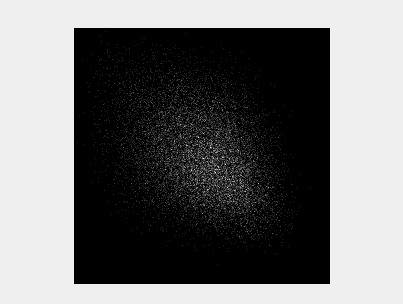
\includegraphics[width=0.7\textwidth, keepaspectratio]{texture_a1.png}\\
  Bild: p09\_teil1\_gras.jpg\\
  Winkel: 0°\\
  Kontrast \approx 1781,44\\
  Entropie \approx 3,9758\\
  Homogenität \approx 0,0746
\end{figure}
\begin{figure}[H]
  \centering
  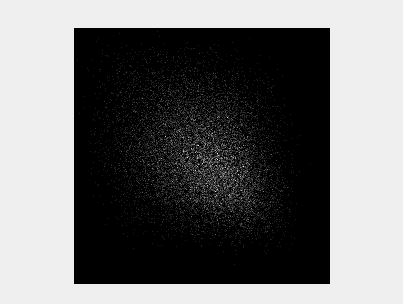
\includegraphics[width=0.7\textwidth, keepaspectratio]{texture_a2.png}\\
  Bild: p09\_teil1\_gras.jpg\\
  Winkel: 45°\\
  Kontrast \approx 2017,27\\
  Entropie \approx 3,9751\\
  Homogenität \approx 0,0725
\end{figure}
\begin{figure}[H]
  \centering
  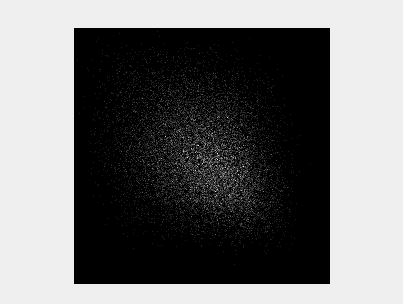
\includegraphics[width=0.7\textwidth, keepaspectratio]{texture_a3.png}\\
  Bild: p09\_teil1\_gras.jpg\\
  Winkel: 90°\\
  Kontrast \approx 2017,26\\
  Entropie \approx 3,9751\\
  Homogenität \approx 0,0725
\end{figure}
\begin{figure}[H]
  \centering
  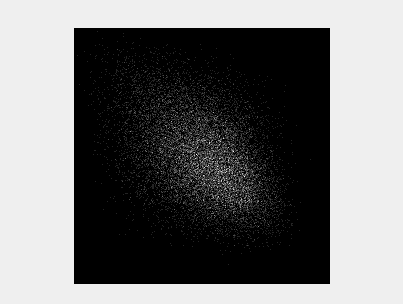
\includegraphics[width=0.7\textwidth, keepaspectratio]{texture_a4.png}\\
  Bild: p09\_teil1\_gras.jpg\\
  Winkel: 135°\\
  Kontrast \approx 1571,17\\
  Entropie \approx 3,9684\\
  Homogenität \approx 0,0806
\end{figure}
\begin{figure}[H]
  \centering
  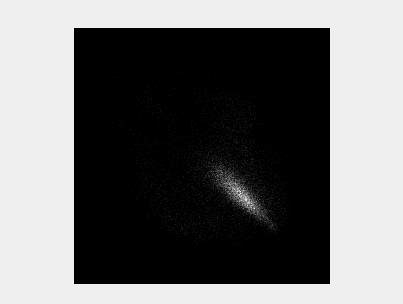
\includegraphics[width=0.7\textwidth, keepaspectratio]{texture_b1.png}\\
  Bild: p09\_teil1\_ziegel.jpg\\
  Winkel: 0°\\
  Kontrast \approx 906,84\\
  Entropie \approx 3,5924\\
  Homogenität \approx 0,1737
\end{figure}
\begin{figure}[H]
  \centering
  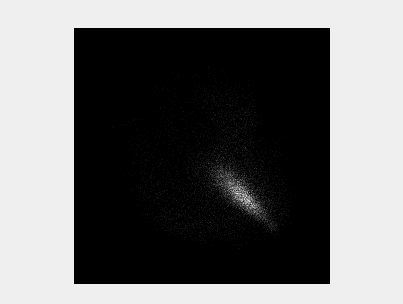
\includegraphics[width=0.7\textwidth, keepaspectratio]{texture_b2.png}\\
  Bild: p09\_teil1\_ziegel.jpg\\
  Winkel: 45°\\
  Kontrast \approx 976,58\\
  Entropie \approx 3,6129\\
  Homogenität \approx 0,1589
\end{figure}
\begin{figure}[H]
  \centering
  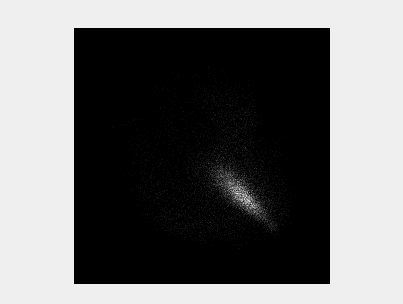
\includegraphics[width=0.7\textwidth, keepaspectratio]{texture_b3.png}\\
  Bild: p09\_teil1\_ziegel.jpg\\
  Winkel: 90°\\
  Kontrast \approx 976,58\\
  Entropie \approx 3,6129\\
  Homogenität \approx 0,1589
\end{figure}
\begin{figure}[H]
  \centering
  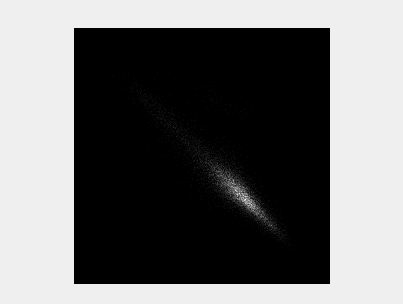
\includegraphics[width=0.7\textwidth, keepaspectratio]{texture_b4.png}\\
  Bild: p09\_teil1\_ziegel.jpg\\
  Winkel: 135°\\
  Kontrast \approx 135,58\\
  Entropie \approx 3,4145\\
  Homogenität \approx 0,238
\end{figure}

\subsection*{Teil 2. PCA für die Dimensionreduktion}
Die Hauptkomponentenanalyse und Dimensionsreduktion ist in der Funktion \textbf{aufgabe\_2} (main.py Zeile 101) implementiert.
In dieser Funktion wird zunächst in den Zeilen 106 bis 123 die Hauptkomponentenanalyse anhand der Trainingsdaten durchgeführt, dabei wird als ergebnis eine Matritze mit Eigenvektoren (\textbf{vh}) erstellt.

Anhand einer Untermenge der Eigenvektoren (20\%, 40\% und 80\%) wird dann in den Zeilen 130 bis 142 die Dimensionsreduktion durchgeführt.

\subsubsection*{Ergebnisbilder}
\begin{figure}[H]
  \centering
  
\includegraphics[width=0.7\textwidth, keepaspectratio]{pca_20.png}\\
  20\% der Eigenvektoren
\end{figure}
\begin{figure}[H]
  \centering
  
\includegraphics[width=0.7\textwidth, keepaspectratio]{pca_40.png}\\
  40\% der Eigenvektoren
\end{figure}
\begin{figure}[H]
  \centering
  
\includegraphics[width=0.7\textwidth, keepaspectratio]{pca_80.png}\\
  80\% der Eigenvektoren
\end{figure}

\end{document}
